
\documentclass[preprint2]{emulateapj}

\usepackage{natbib}
\bibliographystyle{apj}
\usepackage{longtable}
\usepackage[]{graphicx}
\usepackage{amsmath}
\usepackage{natbib}
\usepackage{tabularx}
\usepackage{bm}

%% Sometimes a paper's abstract is too long to fit on the
%% title page in preprint2 mode. When that is the case,
%% use the longabstract style option.

%% \documentclass[preprint2,longabstract]{aastex}

\newcommand{\vdag}{(v)^\dagger}
\newcommand{\myemail}{gsavorgn@astro.swin.edu.au}
\newcommand{\fitfigurewidth}{0.8\textwidth}


\shorttitle{M-M paper}
\shortauthors{Savorgnan et al.}

\begin{document}

\title{M-M paper, morphological bias }

\author{G. A. D. Savorgnan\altaffilmark{1} and A. W. Graham\altaffilmark{1}}
\affil{Centre for Astrophysics and Supercomputing, Swinburne University of Technology, Hawthorn, Victoria 3122, Australia.}
\email{gsavorgn@astro.swin.edu.au}

%\and

%\author{A. W. Graham\altaffilmark{1}}
%\affil{Centre for Astrophysics and Supercomputing, Swinburne University of Technology, Hawthorn, Victoria 3122, Australia.}

%% Notice that each of these authors has alternate affiliations, which
%% are identified by the \altaffilmark after each name.  Specify alternate
%% affiliation information with \altaffiltext, with one command per each
%% affiliation.

%\altaffiltext{1}{Visiting Astronomer, Cerro Tololo Inter-American Observatory.
%CTIO is operated by AURA, Inc.\ under contract to the National Science
%Foundation.}
%\altaffiltext{2}{Society of Fellows, Harvard University.}
%\altaffiltext{3}{present address: Center for Astrophysics,
%    60 Garden Street, Cambridge, MA 02138}
%\altaffiltext{4}{Visiting Programmer, Space Telescope Science Institute}
%\altaffiltext{5}{Patron, Alonso's Bar and Grill}

%% Mark off your abstract in the ``abstract'' environment. In the manuscript
%% style, abstract will output a Received/Accepted line after the
%% title and affiliation information. No date will appear since the author
%% does not have this information. The dates will be filled in by the
%% editorial office after submission.

\begin{abstract}
abstract 
\end{abstract}

\keywords{keywords}

\section{Introduction}
\label{sec:int}
More than two and a half decades ago, 
\cite{dressler1989} foresaw a ``rough scaling of black hole mass with the mass of the spheroidal component'', 
as suggested by the sequence of five galaxies (M87, M104, M31, M32 and the Milky Way). 
His ``rough scaling'' was a premature version of the nowadays popular correlation between black hole mass, $M_{\rm BH}$,  
and host spheroid luminosity, $L_{\rm sph}$, and also host spheroid mass, $M_{\rm sph}$ 
\citep{yee1992,kormendyrichstone1995,magorrian1998,marconihunt2003,haringrix2004}. 
These early studies were dominated by high-mass, early-type galaxies, 
for which they reported a quasi-linear $M_{\rm BH} - M_{\rm sph}$ relation, 
in agreement with a dry-merging formation scenario. 
Subsequent studies of the $M_{\rm BH} - L_{\rm sph}$ and $M_{\rm BH} - M_{\rm sph}$ diagrams 
(\citealt{ferrareseford2005,lauer2007,graham2007,graham2008bar,gultelkin2009,sani2011,beifiori2012,erwingadotti2012,
vika2012,vandenbosch2012,mcconnellma2013,kormendyho2013,rusli2013}; 
see \citealt{graham2015bulges} for an extensive review about the early discovery and successive improvements of these correlations)
used similar galaxy samples, which remained dominated by high-mass, early-type objects having $M_{\rm BH} \gtrsim 0.5 \times 10^8~\rm M_\odot$, 
and therefore recovered a near-linear relation. 
However, the consensus about a linear $M_{\rm BH} - M_{\rm sph}$ correlation was not unanimous. 
Some studies reported a slope steeper than 1,  
or noticed that low-mass spheroids were downwards offset from the relation traced by their high-mass counterparts 
\citep{laor1998,wandel1999,laor2001,ryan2007}.


lasker





 

\section{Data}
\label{sec:data}
\begin{figure}[h]
\begin{center}
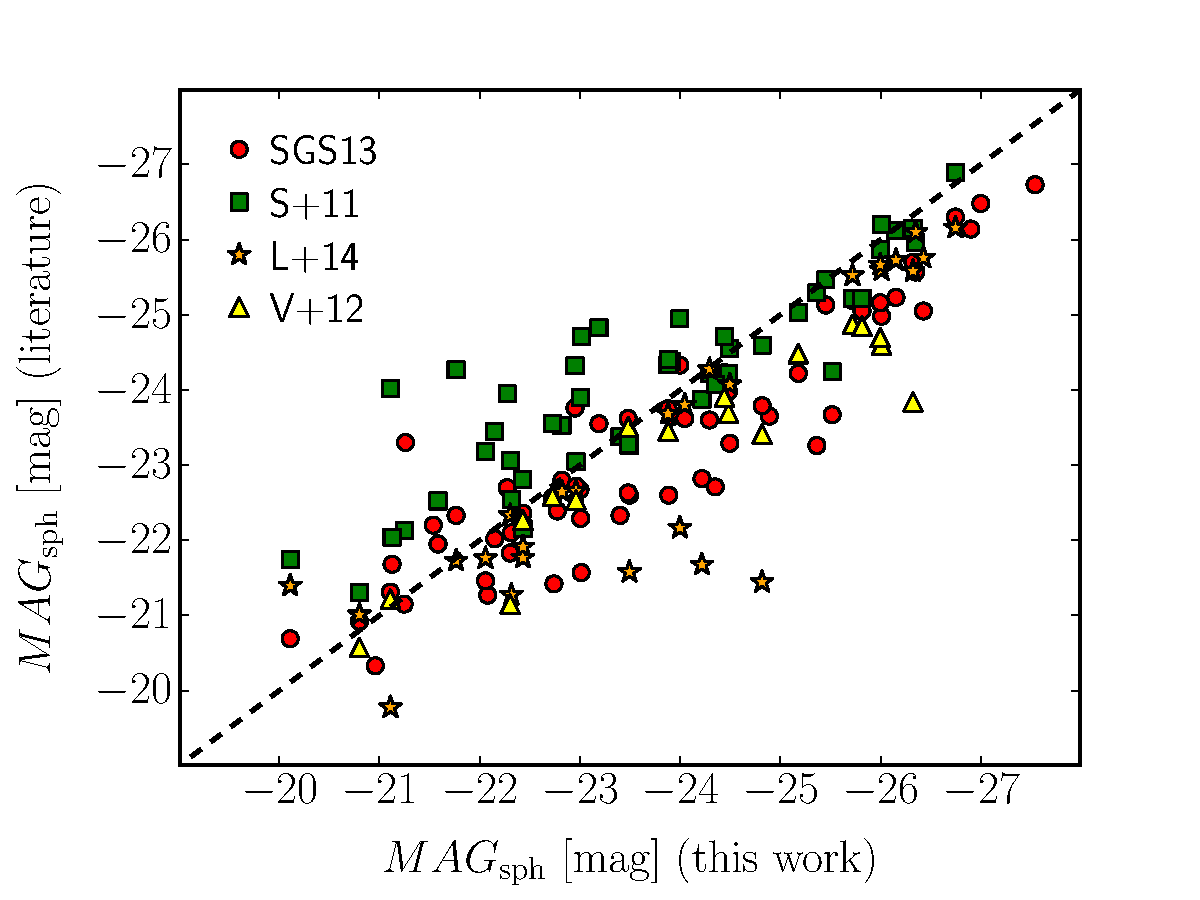
\includegraphics[width=\columnwidth]{images/mag_lit_vs_mag_my.pdf}
\caption{}
\label{fig:}
\end{center}
\end{figure}



\section{Analysis}
\label{sec:anal}
\begin{figure}[h]
\begin{center}
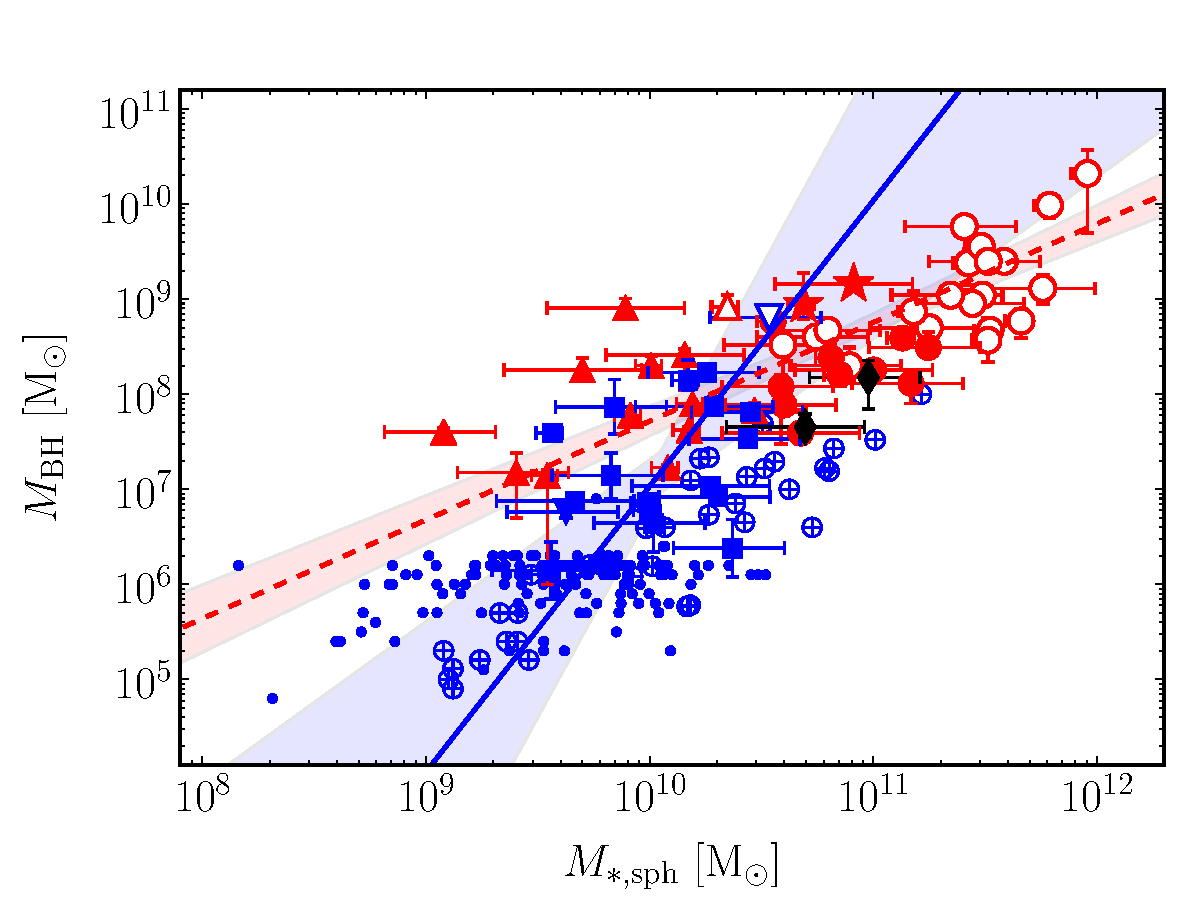
\includegraphics[width=\columnwidth]{images/mbh_vs_mass_sph_agn.pdf}
\caption{}
\label{fig:}
\end{center}
\end{figure}



\section{Results}
\label{sec:res}



\section{Conclusions}
\label{sec:concl}



\acknowledgments
%{\bf marconi, sani, hunt...}
%GS warmly thanks Chieng Peng, Peter Erwin, Luca Cortese, Elisabete Lima Da Cunha and Gonzalo Diaz 
%for useful discussion. \\
This research was supported by Australian Research Council funding through grants
DP110103509 and FT110100263.
This work is based on observations made with the IRAC instrument \citep{fazio2004IRAC} 
on-board the Spitzer Space Telescope, 
which is operated by the Jet Propulsion Laboratory, 
California Institute of Technology under a contract with NASA.
This research has made use of the GOLDMine database \citep{goldmine} and the NASA/IPAC Extragalactic Database (NED) 
which is operated by the Jet Propulsion Laboratory, California Institute of Technology, 
under contract with the National Aeronautics and Space Administration. 


\bibliography{/Users/gsavorgnan/Dropbox_notsync/giulia_e_basta/Literature/SMBHbibliography}


\clearpage


\end{document}

